\section{Description of the model} \label{model}
\subsection{Autoencoders}
Autoencoders are widely used in Deep Learning applications with the main intention
the describe a set of data, mostly targeting dimensionality reduction of creating
a general represenation of the dataset.
This allows the application of such models for anomaly detection, that can be translated
as outlier detection problem in this generated representation,
called feature vector or latent space.
Such approach does not require annotated dataset, therefore belongs to the class of
unsupervised learning algorithms.

The general structure of Autoencoders are shown in Figure \ref{fig:autoencoder}.

\begin{figure}[!ht]
    \centering
    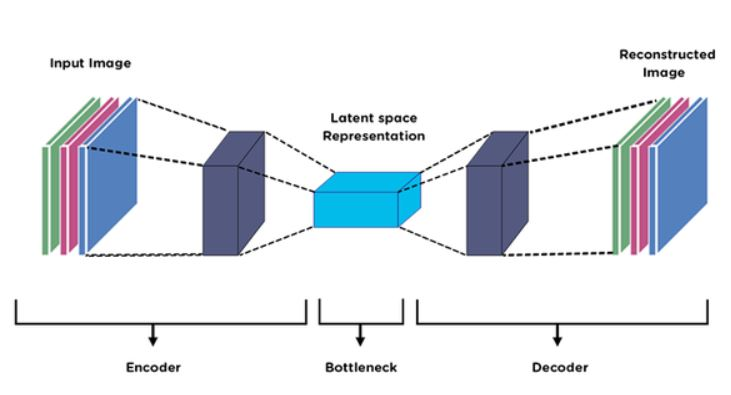
\includegraphics[width=0.6\textwidth]{./tex_images/autoencoder.jpeg}
    \caption{General structure of Autoencoders \cite{khosla_auto_2021}}
    \label{fig:autoencoder}
\end{figure}

A comprehensive overview about Deep Learning methodology is given in \cite{Goodfellow-et-al-2016}.
Chapter 14 of this book explains that mathemathical structure of Autoencoders.
Another introduction can be found at \cite{_autoencoder_2023}.

\subsection{Type of Encoders}
\subsection{Applied Decoder}
\subsection{Basis of anomaly detection}
\subsection{Model training}
\subsection{Performance evaluation}
